\documentclass[tikz,border=3pt]{standalone}
\usepackage[utf8]{inputenc}
\usepackage[T1]{fontenc}
\usepackage{libertinus}
\usepackage{amsmath,amssymb}
\usetikzlibrary{arrows.meta,calc,patterns,decorations.pathmorphing,decorations.markings,decorations.pathreplacing,bending}
\definecolor{UGblue}{RGB}{0,51,102}
\newcommand{\dbar}{\mathchar'26\mkern-12mu d}
\tikzset{
  >=Stealth,
  every node/.style={font=\small},
  caja/.style={draw,line width=0.9pt},
  pared/.style={draw,line width=1.6pt},
  ejes/.style={->,line width=0.8pt},
  adia/.style={draw,pattern=north east lines,pattern color=black!70,line width=0.5pt},
  gas/.style={fill=UGblue!8},
  punto/.style={fill,circle,inner sep=1.3pt},
  onda/.style={decorate,decoration={snake,amplitude=1.1pt,segment length=5pt,post length=3pt,pre length=0pt}},
}
\begin{document}
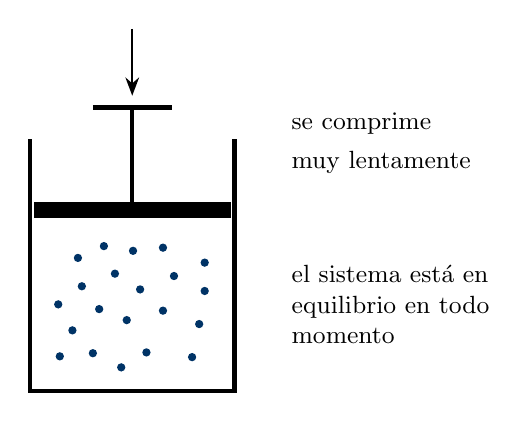
\begin{tikzpicture}
  \draw[pared] (0,3.2) -- (0,0) -- (2.6,0) -- (2.6,3.2);
  \fill[black] (0.05,2.2) rectangle (2.55,2.4);
  \draw[line width=1.6pt] (1.3,2.4) -- (1.3,3.6);
  \draw[line width=1.6pt] (0.8,3.6) -- (1.8,3.6);
  \fill[UGblue] (1.23,0.90) circle (1.5pt);
  \fill[UGblue] (0.61,1.69) circle (1.5pt);
  \fill[UGblue] (0.36,1.10) circle (1.5pt);
  \fill[UGblue] (2.06,0.43) circle (1.5pt);
  \fill[UGblue] (1.40,1.29) circle (1.5pt);
  \fill[UGblue] (1.69,1.02) circle (1.5pt);
  \fill[UGblue] (0.80,0.48) circle (1.5pt);
  \fill[UGblue] (1.31,1.78) circle (1.5pt);
  \fill[UGblue] (1.08,1.49) circle (1.5pt);
  \fill[UGblue] (0.54,0.77) circle (1.5pt);
  \fill[UGblue] (1.48,0.49) circle (1.5pt);
  \fill[UGblue] (0.38,0.44) circle (1.5pt);
  \fill[UGblue] (1.69,1.82) circle (1.5pt);
  \fill[UGblue] (2.22,1.27) circle (1.5pt);
  \fill[UGblue] (2.22,1.63) circle (1.5pt);
  \fill[UGblue] (0.88,1.04) circle (1.5pt);
  \fill[UGblue] (2.15,0.85) circle (1.5pt);
  \fill[UGblue] (1.83,1.46) circle (1.5pt);
  \fill[UGblue] (0.94,1.84) circle (1.5pt);
  \fill[UGblue] (1.16,0.30) circle (1.5pt);
  \fill[UGblue] (0.66,1.33) circle (1.5pt);
  \draw[->,line width=0.8pt] (1.3,4.6) -- (1.3,3.75);
  \node[right] at (3.2,3.4) {se comprime};
  \node[right] at (3.2,2.9) {muy lentamente};
  \node[right,align=left] at (3.2,1.1) {el sistema está en\\equilibrio en todo\\momento};
\end{tikzpicture}
\end{document}
